
\begin{frame}[plain,c]
\begin{center}
{\Huge \bf Optional reading for Lecture \thislecture}
\end{center}
\end{frame}

% ------------------------------------------------------------------------------

%
% Worked example :
%

{
\problemslide

%
%
%

\begin{frame}{Worked example: Current loop on incline}

  \begin{blockexmplque}{Question}
    \begin{minipage}[l]{0.37\textwidth}
     \begin{center}
         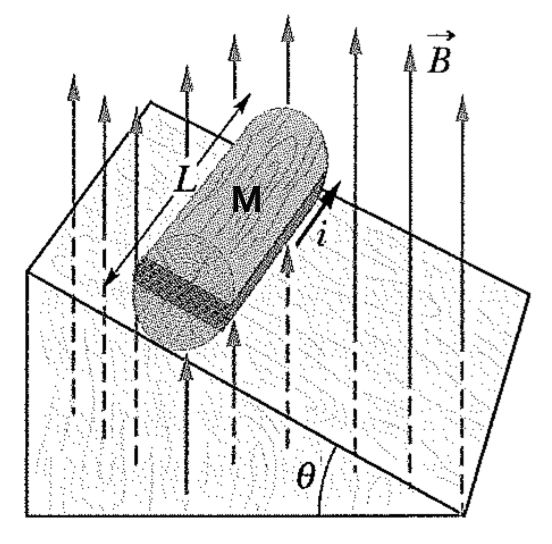
\includegraphics[width=0.80\textwidth]{./images/problems/lect06_cylinder_on_incline}
     \end{center}
    \end{minipage}
    \begin{minipage}[r]{0.60\textwidth}
    	The figure on the left shows a wood cylinder of mass M = 0.250 kg and length
    	L = 0.100 m, with N = 10.0 turns of wire wrapped around it longitudinally,
    	so that the plane of the wire coil contains the long central axis of the cylinder.
    	The cylinder is released on a plane inclined at an angle $\theta$ to the horizontal,
    	with the plane of the coil parallel to the incline plane. If there is a vertical
    	uniform magnetic field of magnitude 0.500 T, what is the least current i through
    	the coil that keeps the cylinder from rolling down the plane?
    \end{minipage}
  \end{blockexmplque}

\end{frame}

%
%
%

\begin{frame}{Worked example: Current loop on incline}

  We take the $x$ axis to be positive down the incline.
  Then the $x$ component of Newton's second law for the center of mass yields:
  \begin{equation*}
  	M g sin\theta - f = M a
  \end{equation*}
  where $f$ is the force of friction, acting up the incline at the point of contact
  $a$ is the cylinder's acceleration, and $M g sin\theta$ is the force of gravity
  in the direction of $x$.

  Since the plane of the loop is parallel to the incline, the dipole moment $\vec{m}$
  is normal to the incline and it has a maginutude of:
  \begin{equation*}
  	|\vec{m}| = I |\vec{S}| = N i L 2r
  \end{equation*}
  where $I$ = $Ni$ is the total current flowing in the loop ($N$ turns of current $i$)
  and $|\vec{S}|$ = $L 2r$ is the area of the loop ($L$ is the length of the cylinder
  and $r$ is its radius).

\end{frame}

%
%
%

\begin{frame}{Worked example: Current loop on incline}

  The magnetic field produces a torque with magnitude:
  \begin{equation*}
  	|\vec{T_B}| = |\vec{m} \times \vec{B}| = |\vec{m}| |\vec{B}| sin\theta
  \end{equation*}

  The force of friction produces a torque with magnitude:
  \begin{equation*}
  	|\vec{T_f}| = f r
  \end{equation*}
  $\vec{T_B}$ produces an angular acceleration in the counterclockwise direction,
  and $\vec{T_f}$ produces an angular acceleration in the clockwise direction.\\

  \vspace{0.2cm}

  Newton's second law for rotation about the center of the cylinder, gives:
  \begin{equation*}
  	|\vec{m}| |\vec{B}| sin\theta - f r = I \alpha
  \end{equation*}
  where $I$ is the mass moment of inertia and
  $\alpha$ is the angular acceleration.\\

\end{frame}

%
%
%

\begin{frame}{Worked example: Current loop on incline}

  Since we want the current that holds the cylinder in place,
  we set $a$ = 0 and $\alpha$ = 0.\\

  \vspace{0.2cm}

  Therefore:
  \begin{equation*}
  	M g sin\theta - f = M a \Rightarrow f = M g sin\theta
  \end{equation*}
  and
  \begin{equation*}
  	|\vec{m}| |\vec{B}| sin\theta - f r = 0 \Rightarrow
  \end{equation*}
  \begin{equation*}
  	( N i L 2r ) |\vec{B}| sin\theta - ( M g sin\theta ) r = 0 \Rightarrow
  \end{equation*}
  \begin{equation*}
  	i = \frac{Mg}{2NLB} \Rightarrow
  \end{equation*}
  \begin{equation*}
  	i = \frac{(0.250 \; kg)(9.8 \; m/s^2)}{2(10.0)(0.100 \; m)(0.500 \; T)} = 2.45 \; A
  \end{equation*}

\end{frame}

} % Worked example

% ------------------------------------------------------------------------------

%
% Worked example :
%

{
\problemslide

%
%
%

\begin{frame}{Worked example: System of 3 wires}

  \begin{blockexmplque}{Question}
    \begin{minipage}[r]{0.75\textwidth}
      Consider 3 straight, infinitely long, coplanar,
      equally spaced wires with zero radius,
      each carrying a current $I$ in the same direction.
      \begin{enumerate}
        \item Find the positions where the magnetic field is zero.
        \item Sketch the magnetic field lines.
        \item If the middle wire is displaced a very small distance $x$
         ($x << d$) to the right (as shown in the diagram)
         while the other 2 wires are held fixed,
         show that it will excecute a simple harmonic oscillation.
         If the wire has linear mass density $\lambda$ (mass per unit length)
         find the angular frequency of oscillation.
      \end{enumerate}
    \end{minipage}
    \begin{minipage}[l]{0.20\textwidth}
     \begin{center}
       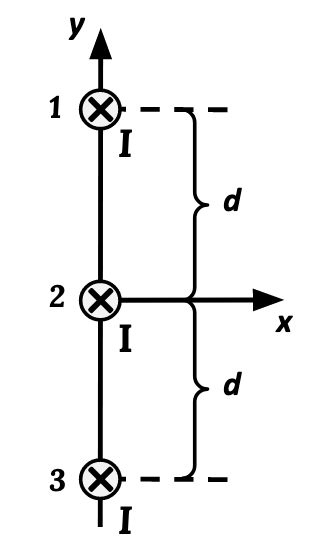
\includegraphics[width=0.94\textwidth]{./images/problems/lect06_3wires_1}
     \end{center}
    \end{minipage}
  \end{blockexmplque}

\end{frame}

%
%
%

\begin{frame}{Worked example: System of 3 wires}

  The magnetic field $\vec{B}$, produced by each long straight wire
  carrying a current $I$, it is azimuthal, and it is given by
  \begin{equation*}
    \vec{B} = \frac{\mu_0 I}{2 \pi r} \hat{\phi}
  \end{equation*}
  where $r$ is the distance from the wire.\\
  \vspace{0.2cm}

  Since the three wires are coplanar, and they carry current in the same direction
  producing similar azimulthal magnetic fields,
  the points of zero magnetic field must be
  located between the wires, and be on the same plane as the wires.
  There must be two zero-field points on each plane perpendicular to the three wires.
  On each such plane, the zero-field points are between the wires and lie on the
  axis that connects the wires.\\
  \vspace{0.2cm}

  Let $y$ be the distance between the middle wire and one of the zero-field points.
  For each such point, the field from the closest
  wire that lies on one side will cancel out the anti-parallel fields from the
  other two wires that lie on the opposite side.

\end{frame}

%
%
%

\begin{frame}{Worked example: System of 3 wires}

  Therefore, we can write:
  \begin{equation*}
      \frac{\mu_0 I}{2\pi(d-y)} = \frac{\mu_0 I}{2\pi y} + \frac{\mu_0 I}{2\pi(d+y)}
  \end{equation*}

  \begin{minipage}[r]{0.55\textwidth}
    The above yields:
    \begin{equation*}
        \frac{1}{d-y} = \frac{1}{y} + \frac{1}{d+y} \Rightarrow
    \end{equation*}
    \begin{equation*}
        \frac{1}{d-y} = \frac{d+2y}{y(d-y)} \Rightarrow
    \end{equation*}
    \begin{equation*}
        y(d+y) = (d-y)(d+2y) \Rightarrow
    \end{equation*}
    \begin{equation*}
        \cancel{yd} + y^2 = d^2 + \cancel{2yd} - \cancel{yd} - 2y^2 \Rightarrow
    \end{equation*}
    \begin{equation*}
        3y^2 = d^2 \Rightarrow
    \end{equation*}
    \begin{equation*}
        y = \pm \frac{d}{\sqrt{3}}
        \label{eq:p3_yvalues_zeroB}
    \end{equation*}
  \end{minipage}
  \begin{minipage}[l]{0.40\textwidth}
    The magnetic field lines, are shown below:
    \begin{center}
      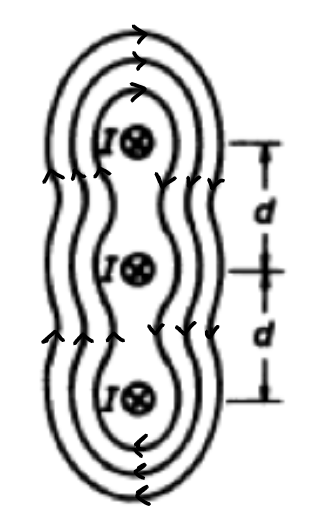
\includegraphics[width=0.50\textwidth]{./images/problems/lect06_3wires_sol_a_1}
    \end{center}
  \end{minipage}

\end{frame}

%
%
%

\begin{frame}{Worked example: System of 3 wires}

  \begin{columns}
    \begin{column}{0.40\textwidth}
      If the middle wire (2) is displaced by a small distance $x$ in the direction of
      the positive $x$ axis, the (attractive) forces $\vec{F}_{21}$ and $\vec{F}_{23}$
      exerted on wire 2 because of wires 1 and 3, correspondingly, are shown in
      the figure on the right.
    \end{column}
    \begin{column}{0.60\textwidth}
      \begin{center}
        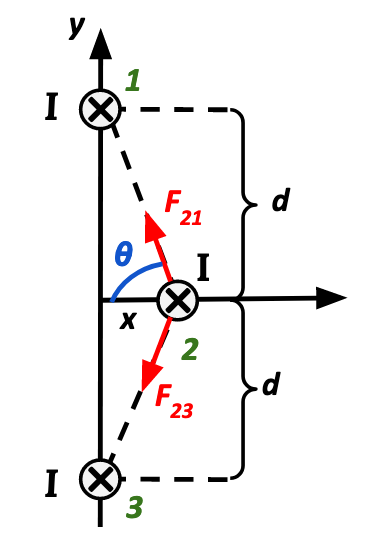
\includegraphics[width=0.70\textwidth]{./images/problems/lect06_3wires_sol_b_1}
      \end{center}
    \end{column}
  \end{columns}

\end{frame}

%
%
%

\begin{frame}{Worked example: System of 3 wires}

  These forces will have the same magnitude, which given by:
  \begin{equation*}
      F_{21} = F_{23} = \frac{\mu_0 I^2}{2\pi \sqrt{d^2+x^2}} L
  \end{equation*}
  where $L$ is the length of the wires.

  As it can be seen, the $y$ components of $\vec{F}_{21}$ and $\vec{F}_{23}$
  cancel out. The (negative) $x$ components of both of these forces
  will contribute to the total force $\vec{F}_{2}$ exerted on wire 2,
  which is given by:
  \begin{equation*}
      \vec{F}_2 = - \Big( F_{21} cos\theta + F_{23} cos\theta \Big) \hat{x}
  \end{equation*}

  Using the expressions we derived for $F_{21}$ and $F_{23}$,
  the above becomes:
  \begin{equation*}
      \vec{F}_2 = - \cancel{2} \frac{\mu_0 I^2}{\cancel{2}\pi \sqrt{d^2+x^2}} L cos\theta \hat{x}
  \end{equation*}

\end{frame}

%
%
%

\begin{frame}{Worked example: System of 3 wires}

  Given that:
  \begin{equation*}
      cos\theta = \frac{x}{\sqrt{d^2+x^2}}
  \end{equation*}
  the previous expression for $\vec{F}_2$ can be written as:
  \begin{equation*}
      \vec{F}_2 = - \frac{\mu_0 I^2}{\pi} \frac{x}{d^2+x^2} L \hat{x} \xRightarrow{d^2+x^2 \approx d^2}
  \end{equation*}

  \begin{equation*}
      \vec{F}_2 = - \frac{\mu_0 I^2 L}{\pi d^2} x \hat{x}
  \end{equation*}

  As it can be seen, the force is proportional and opposite to the
  displacement, Hence the motion of the wire is a simple harmonic oscillation
  about the equilibrium position at $x$=0.

  Using Newton's second law, we can write:
  \begin{equation*}
      \vec{F}_2 = m \frac{d^2 x}{dt^2} \hat{x} \Rightarrow
  \end{equation*}

\end{frame}

%
%
%

\begin{frame}{Worked example: System of 3 wires}

  \begin{equation*}
      - \frac{\mu_0 I^2 L}{\pi d^2} x \hat{x} = m \frac{d^2 x}{dt^2} \hat{x}
      \xRightarrow{m = \lambda L}
  \end{equation*}

  \begin{equation*}
      - \frac{\mu_0 I^2 L}{\pi d^2} x = \lambda L \frac{d^2 x}{dt^2} \Rightarrow
  \end{equation*}

  \begin{equation*}
     \frac{d^2 x}{dt^2} + \frac{\mu_0 I^2}{\pi \lambda d^2} x
  \end{equation*}

  which has the form of the known equation of
  motion for a harmonic oscillator (\"x+$\omega^2$x = 0).
  From this we can deduce that the angular frequency of oscillation, $\omega$,
  is given by:

  \begin{equation*}
     \omega = \sqrt{\frac{\mu_0 I^2}{\pi \lambda d^2}} =
      \frac{I}{d} \sqrt{\frac{\mu_0}{\pi \lambda}}
  \end{equation*}

\end{frame}

} % Worked example

% ------------------------------------------------------------------------------

%
% Worked example :
%

{
\problemslide

%
%
%

\begin{frame}{Worked example: Circular coil in uniform field}

\begin{blockexmplque}{Question}
  A circular coil, 0.05 m in radius, with 30 turns of wire, lies on the horizontal plane.
  It carries a current of 5.0 A counterclockwise (as viewed from the top).
  The coil is in a uniform magnetic field of 1.2 T directed to the right.
  Find the magnetic moment and the torque on the coil in vector form.
\end{blockexmplque}

The magnetic dipole moment $\vec{m}$ of a current loop is defined as:
\begin{equation*}
   \vec{m} = I \vec{S}
\end{equation*}
where I is the current flowing in the loop and $\vec{S}$ is its area.

The area of a circular coil with radius r = 0.05 m is
\begin{equation*}
  S = \pi r^2 = \pi (0.05\; m)^2 = 0.00785 \; m^2
\end{equation*}

The current $I_{turn}$ flowing through each turn of wire is 5.0 A
and the coil has N = 30 turns. Hence, the total current is:
\begin{equation*}
  I = N I_{turn} = 30 \cdot 5\; A = 150 \; A
\end{equation*}

\end{frame}

%
%
%

\begin{frame}{Worked example: Circular coil in uniform field}

Therefore, the magnitude of the magnetic moment $\vec{m}$ is:
\begin{equation*}
   |\vec{m}| = I \cdot S = \Big(  150 \; A \Big) \cdot \Big( 0.00785 \; m^2 \Big) \approx 1.18 \; A \cdot m^2
\end{equation*}

The vector $\vec{m}$ is perpendicular to the loop and points in the same
direction as your thumb if your right-hand curls in the direction of the current.
The given circular coil lies on the horizontal plane
(which we assume to be the $xy$ plane, with $x$ pointing on the right)
with $I$ flowing counterclockwisely.\\

\vspace{0.1cm}
Therefore, the direction of the magnetic moment is along $\hat{z}$:
\begin{equation*}
   \vec{m} \approx \Big( 1.18 \; A \cdot m^2 \Big) \hat{z}
\end{equation*}

The torque exerted by a magnetic field is:
\begin{equation*}
     \vec{T} = \vec{m} \times \vec{B} \Rightarrow
\end{equation*}
\begin{equation*}
     \vec{T}
     = \Big( 1.18 \; A \cdot m^2 \Big) \hat{z} \times \Big( 1.2 \; T \Big) \hat{x}
     \approx \Big( 1.42 \; N \cdot m \Big) \Big( \hat{z} \times \hat{x} \Big)
     = \Big( 1.42 \; N \cdot m \Big) \hat{y}
\end{equation*}

\end{frame}

} % Worked example

% ------------------------------------------------------------------------------

%
% Worked example :
%

{
\problemslide

%
%
%

\begin{frame}{Worked example: Magnetic field of cylindrical conductor}

  \begin{blockexmplque}{Question}
    A long non-magnetic cylindrical conductor with inner radius $a$
    and outer radius $b$ carries a current $I$ which flows along the
    direction of the axis of symmetry of the cylinder.
    Assume that the current density in the conductor is uniform.\\
    \vspace{0.2cm}
    The current $I$ produces a magnetic field $\vec{B}$.
    Find the magnetic field $\vec{B}$ as a function of the radial
    co-ordinate $r$ and express it in vector form for the following cases:\\
    \vspace{0.2cm}
    \begin{itemize}
       \item inside the hollow space ($r < a$),
       \item within the cylindrical conductor ($a < r < b$), and
       \item outside the conductor ($r > a$).
     \end{itemize}
  \end{blockexmplque}

\end{frame}

%
%
%

\begin{frame}{Worked example: Magnetic field of cylindrical conductor}

  For the calculation of the magnetic field in this cylindrically-symmetric
  problem we will use Ampere's circuital law for a closed path $L$
  \begin{equation*}
     \oint_{L} \vec{B} \cdot d\vec{\ell} = \mu_0 I_{enc}
  \end{equation*}

  where $I_{enc}$ is the current that flows through the open surface $S(L)$
  that has the closed path $L$ as its boundary:
  \begin{equation*}
     I_{enc} = \int_{S(L)} \vec{j} \cdot d\vec{S}
  \end{equation*}

  The uniform current density $j$, within the conductor,
  can be written as the ratio of the
  total current $I$ over the area of a cross-section of the cylinder
  perpendicular to the direction of the current flow.
  If the axis of the cylinder is the $z$ axis, and the current flows
  in the positive direction, we can write:
  \begin{equation*}
     \vec{j} = \frac{I}{\pi(b^2-a^2)} \hat{z} \;\;\;\;\; (\text{for } a < r < b)
  \end{equation*}

\end{frame}

%
%
%

\begin{frame}{Worked example: Magnetic field of cylindrical conductor}

  For {\em any} closed path $L$ in the region $r<a$,
  $I_{enc}$ = 0. Ampere's law yields:
  \begin{equation*}
     \oint_{L} \vec{B} \cdot d\vec{\ell} = 0
  \end{equation*}
  Since this is true for any arbitrary closed path, it can not be the
  result of an accidental cancellation and it has to be the
  integrand itself that is zero.\\
  Therefore, for $r<a$:
  \begin{equation*}
     B = 0
  \end{equation*}
  For $a<r<b$, in order to exploit the cylindrical symmetry of the problem
  in the application of Ampere's law, we choose a circular integration path $L$
  with radius $r$ whose centre is on the symmetry axis of the cylinder.\\
  The current $I_{enc}$ that flows through the area $S$ of a circle
  that has $L$ as its boundary and it is perpendicular to $\vec{j}$,
  is given by:\\
  \begin{equation*}
     I_{enc} = \int_{S(L)} \vec{j} \cdot d\vec{S} = jS =
       I \frac{r^2-a^2}{b^2-a^2}
  \end{equation*}

\end{frame}

%
%
%

\begin{frame}{Worked example: Magnetic field of cylindrical conductor}

  Substituting the above in Ampere's circuital law,
  and considering that, due to symmetry, $\vec{B}$ is an azimuthal vector
  and, along $L$, the vectors $\vec{B}$ and $d\vec{\ell}$
  are co-linear, we obtain:
  \begin{equation*}
     B 2\pi r = \mu_0 I \frac{r^2-a^2}{b^2-a^2} \Rightarrow
     B = \frac{\mu_0 I}{2\pi r} \frac{r^2-a^2}{b^2-a^2}
  \end{equation*}
  Therefore, for $a<r<b$:
  \begin{equation*}
     \displaystyle
     \vec{B} = \frac{\mu_0 I}{2\pi r} \frac{r^2-a^2}{b^2-a^2} \hat{\phi}
  \end{equation*}

  For $r>b$, we can use similar procedure and arguments
  as in the case of $a<r<b$, but with:
  \begin{equation*}
     I_{enc} = I
  \end{equation*}
  since our integration path includes the full cylindrical conductor.
  % An application of Ampere's circuital law in this case yields
  % \begin{equation*}
  %    B 2\pi r = \mu_0 I \Rightarrow
  %    B = \frac{\mu_0 I}{2\pi r}
  % \end{equation*}
  Therefore, for $r>b$:
  \begin{equation*}
     \displaystyle
     \vec{B} = \frac{\mu_0 I}{2\pi r} \hat{\phi}
  \end{equation*}

\end{frame}

} %Worked example

% ------------------------------------------------------------------------------
{
\problemslide

%
%
%

\begin{frame}{Worked example: Magnetic flux through half cylinder}

  \begin{blockexmplque}{Question}
    Two wires, parallel to a z axis and a distance 4$r$ apart,
    carry equal currents $i$ in opposite directions, as shown below.
    A circular cylinder of radius $r$ and length $L$ has its axis on the z axis,
    midway between the wires. Use Gauss' law for magnetism to derive an expression
    for the net outward magnetic flux through the half of the cylindrical
    surface above the x axis.\\
    \begin{center}
        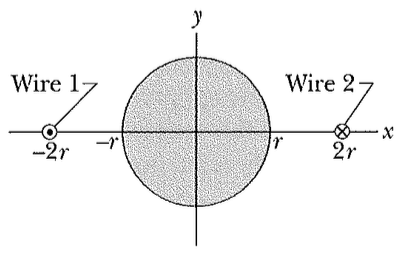
\includegraphics[width=0.50\textwidth]{./images/problems/lect06_2_wires_magnetic_flux_half_cylinder}
    \end{center}
  \end{blockexmplque}

\end{frame}

%
%
%

\begin{frame}{Worked example: Magnetic flux through half cylinder}

  Let S$_1$ be the half of the cylindrical surface (above the x axis) for which
  we are interested in calculating the magnetic flux, and
  S$_2$ be the portion of the xz plane that lies within the cylinder.\\
  \vspace{0.2cm}
  Each of the wires 1 and 2 produces an azimulthal magnetic field, as shown on
  the figure below. The total magnetic field has no z component.

  \begin{center}
      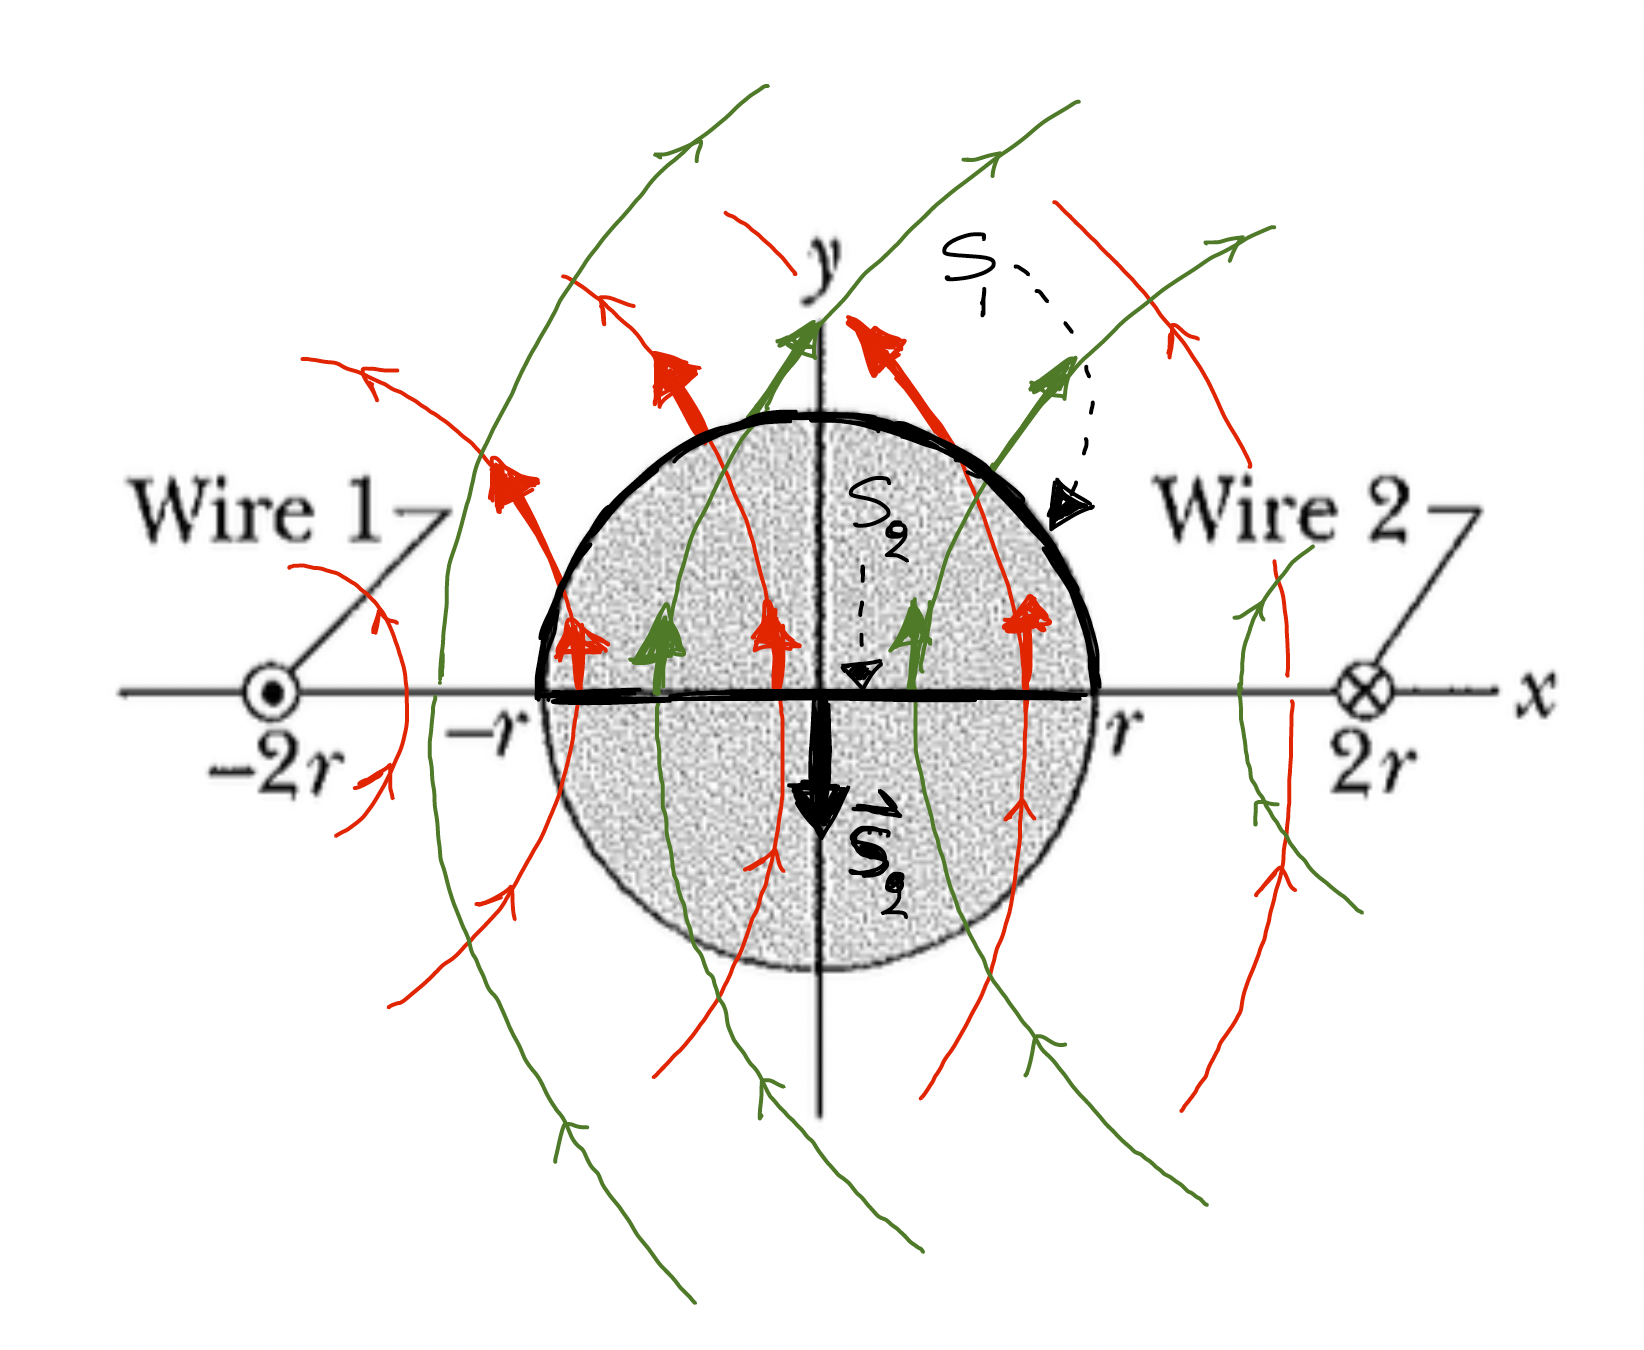
\includegraphics[width=0.50\textwidth]{./images/problems/lect06_2_wires_magnetic_flux_half_cylinder_2}
  \end{center}

\end{frame}

%
%
%

\begin{frame}{Worked example: Magnetic flux through half cylinder}

  From Gauss' law for magnetism, the flux through the closed surface formed by
  S$_1$, S$_2$ and two end-cups on the $xy$ plane (through which there
  is no flux, since the field of each wire is azimuthal) is zero. Therefore:
  \begin{equation*}
  	 \Phi_{S_1} + \Phi_{S_2} = 0 \Rightarrow \Phi_{S_1} = -\Phi_{S_2}
  \end{equation*}

  So we can obtain the flux through the half-cylindrical surface S$_1$, by calculating the
  flux through the planar surface S$_2$. The latter is a much easier calculation.

  The total magnetic flux through the surface S$_2$ is given by
  \begin{equation*}
  	\Phi_{S_2} = \int_{S_2} \vec{B} \cdot d\vec{S}
  \end{equation*}

  The total field $\vec{B}$ is the superposition of the fields $\vec{B}_1$ and
  $\vec{B}_2$ produced by the wires 1 and 2 respectively.
  \begin{equation*}
  	\vec{B} = \vec{B}_1 + \vec{B}_2
  \end{equation*}

\end{frame}

%
%
%

\begin{frame}{Worked example: Magnetic flux through half cylinder}

  The field produced by a long straight wire with current $I_k$ is given by
  \begin{equation*}
     \vec{B}_{k} = \frac{\mu_0 I_k}{2\pi r_k} \hat{\phi_k}
  \end{equation*}
  where $r_k$ is the distance from the wire and $\hat{\phi_k}$
  is the azimuthal direction around that wire.\\
  \vspace{0.1cm}
  The current in wire 1 travels along $\hat{z}$ (out of the page) and therefore
  its magnetic field, as viewed from above, rotates anticlockwisely.
  On the surface S$_2$, the field $\vec{B}_{1}$ points along $\hat{y}$.
  Similarly,
  the current in wire 2 travels along -$\hat{z}$ (into the page) and therefore
  its magnetic field, as viewed from above, rotates clockwisely.
  On the surface S$_2$, the field $\vec{B}_{2}$ points along $\hat{y}$ too.\\
  \vspace{0.1cm}
  So, in summary, on the surface S$_2$:
  \begin{equation*}
     \vec{B}_{1} = \frac{\mu_0 i}{2\pi r_1} \hat{y} = \frac{\mu_0 i}{2\pi (2r+x)} \hat{y}
     \;\;\;\;\; \text{and} \;\;\;\;\;
     \vec{B}_{2} = \frac{\mu_0 i}{2\pi r_2} \hat{y} = \frac{\mu_0 i}{2\pi (2r-x)} \hat{y}
  \end{equation*}

\end{frame}

%
%
%

\begin{frame}{Worked example: Magnetic flux through half cylinder}

  By convention, the unit vector for each element of a closed surface points outwards,
  so the surface vector of S$_2$ points towards -$\hat{y}$.
  Therefore, $\Phi_{S_2}$ is:

  \begin{equation*}
  	\Phi_{S_1} =
  	- \Phi_{S_2} =
  	- \int_{S_2} (\vec{B}_1 + \vec{B}_2) \cdot d\vec{S}
  \end{equation*}

  \begin{equation*}
  	= \frac{\mu_0 i L}{2\pi}
  	   \big\{
  		   \int_{-r}^{+r} \frac{dx}{2r+x} +
  			 \int_{-r}^{+r} \frac{dx}{2r-x}
  	   \big\}
    = \frac{\mu_0 i L}{2\pi}
  	   \big\{
  		   \int_{-r}^{+r} \frac{d(2r+x)}{2r+x} -
  			 \int_{-r}^{+r} \frac{d(2r-x)}{2r-x}
  	   \big\}
  \end{equation*}

  \begin{equation*}
  	=
  	   \frac{\mu_0 i L}{2\pi}
  	   \big\{
  		   ln(2r+x) \rvert_{-r}^{+r} -
  			 ln(2r-x) \rvert_{-r}^{+r}
  	   \big\}
  \end{equation*}
  \begin{equation*}
  	=
  		 \frac{\mu_0 i L}{2\pi}
  		 \big\{
  		   (ln(3r) - ln(r)) -
  			 (ln(r) - ln(3r)
  	   \big\}
  	= \frac{\mu_0 i L}{2\pi}
  		  (2ln(3r) - 2ln(r))
    = \frac{\mu_0 i L}{2\pi} 2 ln3 \Rightarrow
  \end{equation*}

  \begin{equation*}
  	\Phi_{S_1} =
  	    \frac{\mu_0 i}{\pi} L ln3
  \end{equation*}


\end{frame}

} %Worked example


% ------------------------------------------------------------------------------

%
% Worked example :
%

{
\problemslide

%
%
%

\begin{frame}{Worked example: Magnetic forces between 5 parallel wires}

  \begin{blockexmplque}{Question}
    In the figure below, five long parallel wires in an $xy$ plane are separated
    by distance $d$, have lengths $L$, and carry identical currents $I$ out of the page.
    Each wire experiences a magnetic force due to the currents in the other wires.\\
    \begin{center}
        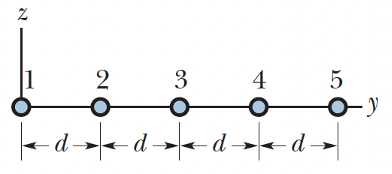
\includegraphics[width=0.45\textwidth]{./images/problems/lect06_5_parallel_wires.png}
    \end{center}
    \vspace{0.2cm}
    In unit vector notation, what is the net magnetic force on
    i) wire 1, ii) wire 2, iii) wire 3, iv) wire 4 and v) wire 5?
  \end{blockexmplque}

\end{frame}

%
%
%

\begin{frame}{Worked example: Magnetic forces between 5 parallel wires}

  The force between 2 parallel straight wires $i$ and $j$ of length $L$,
  carrying currents $I_i$ and $I_j$ respectively, is given by
  \begin{equation*}
    |\vec{F}_{ij}| = \frac{\mu_0 I_{i} I_{j} L}{2 \pi r}
  \end{equation*}
  The force is attractive if the currents have the same direction,
  and repulsive if they have opposite direction. \\

  \vspace{0.2cm}
  Using the superposition principle, we can write the total magnetic force
  $\vec{F}_{1}$ on wire 1, as:
  \begin{equation*}
    \vec{F}_{1} = \vec{F}_{12} + \vec{F}_{13} + \vec{F}_{14} + \vec{F}_{15}
  \end{equation*}
  where $\vec{F}_{1j}$ ($j$=2,3,4,5) is the force on wire 1 due to wire $j$.\\

  \vspace{0.2cm}
  Using the earlier expression for the magnetic force between wires, we find:
  \begin{equation*}
    \vec{F}_{1} =
      \frac{\mu_0 I^2 L}{2 \pi}
      \Big( \frac{1}{d} + \frac{1}{2d} + \frac{1}{3d} + \frac{1}{4d} \Big) \hat{y} =
      \frac{25 \mu_0 I^2 L}{24 \pi d} \hat{y}
  \end{equation*}

\end{frame}

%
%
%

\begin{frame}{Worked example: Magnetic forces between 5 parallel wires}

  Similarly, for wire 2, we have:
  \begin{equation*}
    \vec{F}_{2} = \vec{F}_{21} + \vec{F}_{23} + \vec{F}_{24} + \vec{F}_{25} \Rightarrow
  \end{equation*}

  \begin{equation*}
    \vec{F}_{2} =
      \frac{\mu_0 I^2 L}{2 \pi}
      \Big( - \frac{1}{d} + \frac{1}{d} + \frac{1}{2d} + \frac{1}{3d} \Big) \hat{y} =
      \frac{5 \mu_0 I^2 L}{12 \pi d} \hat{y}
  \end{equation*}

  \vspace{0.2cm}

  From the symmetry of the problem, we see that
  the magnetic force on wire 3 due to the wires 1,2
  has the same magnitude as the  force on wire 3 due to the wires 4,5
  but opposite direction. Therefore:
  \begin{equation*}
    \vec{F}_{3} = \vec{0}
  \end{equation*}

  Sumilarly, due to the symmetry of the problem, we have:
  \begin{equation*}
    \vec{F}_{4} = - \vec{F}_{2} = - \frac{5 \mu_0 I^2 L}{12 \pi d} \hat{y}
  \end{equation*}

  \begin{equation*}
    \vec{F}_{5} = - \vec{F}_{1} = - \frac{25 \mu_0 I^2 L}{24 \pi d} \hat{y}
  \end{equation*}

\end{frame}

} %Worked example

% ------------------------------------------------------------------------------

%
% Worked example :
%

{
\problemslide

%
%
%

\begin{frame}{Worked example: Magnetic moment of 2 concentric loops}

  \begin{blockexmplque}{Question}
    \begin{columns}
      \begin{column}{0.65\textwidth}
          Two concentric, circular wire loops of radii $r_1$ = 20 cm and $r_2$ = 30 cm,
          are located in an $xy$ plane. Each wire loop carries a clockwise current $I$ = 7 A.
          \begin{itemize}
           \item  Find the magnitude of the net magnetic dipole moment of the system.
           \item If the current in the inner loop is reversed, what is the new
           magnitude of the net magnetic dipole moment of the system?
          \end{itemize}
      \end{column}
      \begin{column}{0.35\textwidth}
        \begin{center}
            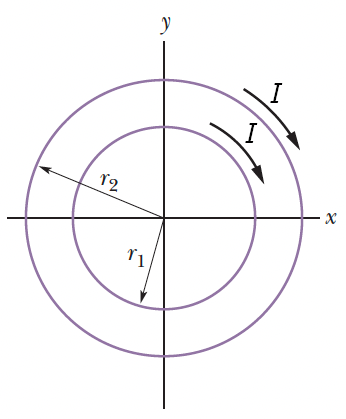
\includegraphics[width=0.95\textwidth]{./images/problems/lect06_2_concentric_wire_loops.png}
        \end{center}
      \end{column}
    \end{columns}
  \end{blockexmplque}

\end{frame}

%
%
%

\begin{frame}{Worked example: Magnetic moment of 2 concentric loops}

  The magnetic dipole moment $\vec{m}$ of circular loop on the $xy$
  plane, with a current $I$ running counterclockwise (as viewed
  from a point in the positive $z$ axis), is given by:
  \begin{equation*}
    \vec{m} = I \vec{S} = I \pi r^2 \hat{z}
  \end{equation*}

  The magnetic dipole moments of the two concentric circular loops
  can be superimposed:
  \begin{equation*}
    \vec{m} = \vec{m}_1 + \vec{m}_2
  \end{equation*}

  Therefore, the net magnetic dipole of the system
  is given by:
  \begin{equation*}
    \vec{m} = \vec{m}_1 + \vec{m}_2
            = \Big(-I \pi r^2_1 - I \pi r^2_2 \Big) \hat{z}
            = (-2.86 \; A m^2) \hat{z}
  \end{equation*}

  If the current of the inner loop is reversed,
  the net magnetic dipole of the system becomes:
  \begin{equation*}
    \vec{m} = \vec{m}_1 + \vec{m}_2
            = \Big(+I \pi r^2_1 - I \pi r^2_2 \Big) \hat{z}
            = (-1.10 \; A m^2) \hat{z}
  \end{equation*}

\end{frame}


} %Worked example

% ------------------------------------------------------------------------------
